% BDE Guide --- Chapter 1: What Is a BDE? (0->100 ground-up)
\chapter{What Is a Broadening \& Deepening Elective?}
\label{ch:bde-overview}

\begin{quote}
\emph{``A computer scientist is someone who knows breadth --- and chooses depth deliberately.''}
BDEs are NTU's formal mechanism for that choice: 20 AU of curated freedom outside your Programme Core and MPE.
\end{quote}

\noindent\fbox{\parbox{\dimexpr\linewidth-2\fboxsep-2\fboxrule}{%
\textbf{From zero: no prior NTU jargon assumed.} We define Academic Unit (AU), curriculum buckets, and every acronym (BDE, MPE, ICC, CSL, GER) from scratch. If you are in Y1 Week~1, start here.}}
\vspace{0.4em}

\section*{Learning Outcomes}
After this chapter you will be able to:
\begin{enumerate}[label=(L\arabic*)]
    \item define AU, BDE, MPE, University Core, and College Core and state the 135~AU total;
    \item explain \emph{why} BDEs exist (breadth vs.\ depth) and where the 20~AU sits in the degree;
    \item list the major BDE categories and give an example course for each;
    \item distinguish GER-PE, GER-UE, and BDE counting rules at a high level;
    \item locate the authoritative sources (Degree Audit, curriculum page, NTUMods) for your cohort.
\end{enumerate}

% ============================================================
\section{Why BDEs Exist: Breadth, Depth, and Choice}
\label{sec:why-bde}

Picture your degree as a fixed 135~AU ``pie''. About 60\% is decided for you --- University Core (17~AU) + College Core (16~AU) + Programme Core (47~AU) --- and another 35~AU is semi-decided (MPE, from an SC3xxx/SC4xxx list). The remaining slice --- about 15\% --- is \emph{yours to design}. That slice is the Broadening \& Deepening Electives (BDE) bucket: 20~AU (curriculum-page counting; the alternative Foundational-Core bucketing in the AY2024--25 PDF summary shows 21~AU for the same total --- the 1~AU delta is a boundary shift between College Core and BDE, not extra workload; the 135~AU total is invariant).

``Broadening'' means stepping outside Computing --- business, psychology, language, art, sustainability. ``Deepening'' means going deeper within or adjacent to Computing but beyond the prescribed list --- e.g., an extra CC000X-adjacent tech-and-society module or a Nanyang Business School analytics elective that complements your MPE. In practice most students blend both.

\begin{definition}[Academic Unit (AU)]
One AU $=$ roughly 13 hours of total learning effort (lectures + tutorials + labs + self-study + assessment) over one 13-week semester. A 3~AU course $\approx$ 39 hours; a 4~AU course $\approx$ 52 hours. Your degree requires 135~AU for the single-degree BSc (Hons) in Computer Science (direct honours, 4 years). Variants --- second major, double degree, University Scholars Programme --- shift AU between buckets but keep the total fixed; confirm via Degree Audit.
\end{definition}

\begin{definition}[BDE vs.\ MPE --- one sentence]
A \emph{Major Prescribed Elective (MPE)} must be an SC3xxx or SC4xxx module from the CCDS MPE list (9 courses, $\ge$4 at 4000-level; FYP path includes SC4079). A \emph{Broadening \& Deepening Elective (BDE)} is any NTU-approved elective not already counted in University/College/Programme Core or MPE. The same course cannot count twice.
\end{definition}

\begin{remark}[Old terminology: GER-PE / GER-UE]
Before AY2021, NTU used General Education Requirement (GER) labels: GER-Core, GER-PE (Prescribed Elective), GER-UE (Unrestricted Elective). UEs are essentially today's BDEs; PEs overlapped with today's MPE + some ICC. If a senior tells you ``use your UEs for BDE'', they mean the same bucket. This guide uses post-AY2021 language (BDE/MPE/ICC) throughout.
\end{remark}

% ============================================================
\section{The 135~AU Map and Where BDEs Sit}
\label{sec:au-map}

\begin{figure}[h]
\centering
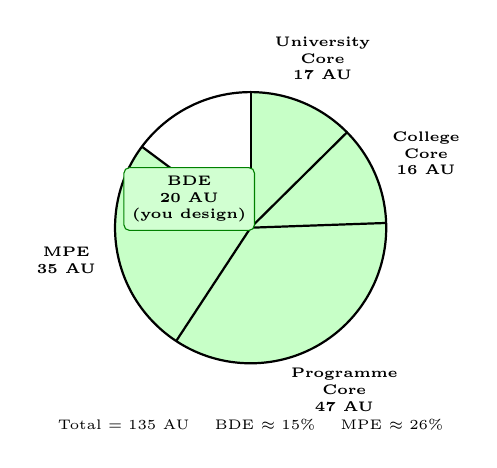
\begin{tikzpicture}[scale=0.82,every node/.style={font=\scriptsize}]
% Pie slices (roughly to scale: 17/16/47/35/20)
\def\r{2.1}
% angles: start at 90deg, clockwise
% University 17/135 = 45.3 deg, College 16/135=42.7, Prog 47/135=125.3, MPE 35/135=93.3, BDE 20/135=53.3
% We'll approximate with filled wedges
\fill[blue!22] (0,0) -- (90:\r) arc (90:44.7:\r) -- cycle;
\fill[teal!22] (0,0) -- (44.7:\r) arc (44.7:2.0:\r) -- cycle;
\fill[orange!22] (0,0) -- (2.0:\r) arc (2.0:-123.3:\r) -- cycle;
\fill[violet!18] (0,0) -- (-123.3:\r) arc (-123.3:-216.7:\r) -- cycle;
\fill[green!22] (0,0) -- (-216.7:\r) arc (-216.7:90:\r) -- cycle;
\draw[thick] (0,0) circle (\r);
\foreach \a in {90,44.7,2.0,-123.3,-216.7} \draw[thick] (0,0) -- (\a:\r);
% labels outside
\node[align=center,font=\tiny\bfseries] at (67:2.85) {University\\Core\\17 AU};
\node[align=center,font=\tiny\bfseries] at (23:2.95) {College\\Core\\16 AU};
\node[align=center,font=\tiny\bfseries] at (-60:2.9) {Programme\\Core\\47 AU};
\node[align=center,font=\tiny\bfseries] at (-170:2.9) {MPE\\35 AU};
\node[fill=green!18,rounded corners=2pt,inner sep=3pt,align=center,font=\tiny\bfseries,draw=green!50!black] at (155:1.05) {BDE\\20 AU\\\tiny (you design)};
\node[font=\tiny,align=center] at (0,-3.05) {Total $=135$ AU  \quad BDE $\approx 15\%$ \quad  MPE $\approx 26\%$};
\end{tikzpicture}
\caption{The 135~AU pie for single-degree CSC (curriculum-page bucketing). Two bucketings exist: curriculum page (ICC+CSL 17 + College 16 + Programme 47 + MPE 35 + BDE 20) and PDF Foundational-Core summary (Core 47 + MPE 35 + ICC 17 + F-Core 15 + BDE 21); both sum to 135. Degree Audit is authoritative for your cohort.}
\label{fig:au-pie}
\end{figure}

Table~\ref{tab:au-buckets} in the Appendix gives the same breakdown in tabular form with both bucketings side-by-side. Key intuition: BDEs are the \emph{only} bucket where essentially any NTU course qualifies (subject to prerequisites and exclusion rules). They are also the bucket most often repurposed if you add a second major or minor --- the second-major's required courses replace BDE AU one-for-one, shrinking free choice.

\subsection{What Counts as a BDE?}
Formally, any NTU course that (i)~carries AU, (ii)~is not already satisfying University Core, College Core, Programme Core, or MPE for your degree, and (iii)~is approved as a BDE in the NTU Course Catalogue is eligible. In practice:

\begin{itemize}
    \item Language courses (LC5001 Chinese, LJ5001 Japanese, LK5001 Korean, LF5001 French, \dots) --- 3--4~AU each.
    \item Business \& management (AB1601 Organisational Behaviour, AB1202 Statistics \& Analysis, AC1103 Accounting, \dots).
    \item Humanities, arts \& social sciences (HP1000 Intro to Psychology, HP8001 Thinking \& Reasoning, HAxxxx Art History, \dots).
    \item Science \& sustainability outside core (CM8001 Energy, BS8003 Science of Food, \dots).
    \item Any SC-coded course \emph{not} on the MPE list or not counted as Programme Core --- rare, but possible (e.g., SC1006-level service modules for non-majors, if offered to CS).
    \item Entrepreneurship \& innovation (ET9131 Entrepreneurship, \dots), physical education electives, and Nanyang Technopreneurship Centre modules.
\end{itemize}

What does \emph{not} count: retaking a course you already passed (no new AU), a course whose content overlaps $>$50\% with one you already took (exclusion list), or the same AU counted in two buckets (no double-counting --- see \S\ref{sec:double-count-intro}).

\subsection{Double-Counting: First Taste}
\label{sec:double-count-intro}
The single most common BDE mistake is ``double-counting'':

\begin{center}
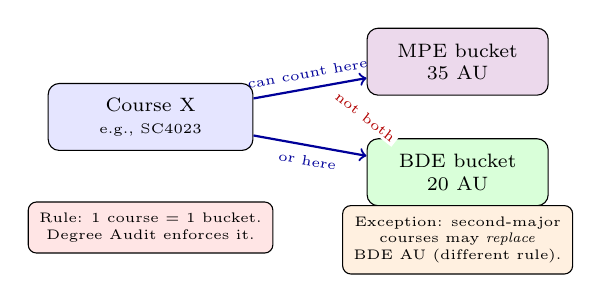
\begin{tikzpicture}[scale=0.78,every node/.style={font=\scriptsize}]
\node[draw,rounded corners=4pt,fill=blue!10,minimum width=2.6cm,minimum height=0.85cm,align=center] (a) at (0,0) {Course X\\{\tiny e.g., SC4023}};
\node[draw,rounded corners=4pt,fill=violet!15,minimum width=2.3cm,minimum height=0.85cm,align=center] (b) at (5.0,0.9) {MPE bucket\\35 AU};
\node[draw,rounded corners=4pt,fill=green!15,minimum width=2.3cm,minimum height=0.85cm,align=center] (c) at (5.0,-0.9) {BDE bucket\\20 AU};
\draw[->,thick,blue!60!black] (a) -- (b) node[midway,above,font=\tiny,sloped] {can count here};
\draw[->,thick,blue!60!black] (a) -- (c) node[midway,below,font=\tiny,sloped] {or here};
\draw[thick,red!70!black] (3.2,0.35) -- (3.8,-0.35) node[midway,fill=white,inner sep=1pt,font=\tiny,rotate=-38] {not both};
\node[draw,rounded corners=3pt,fill=red!10,inner sep=4pt,align=center,font=\tiny] at (0,-1.8) {Rule: 1 course $=$ 1 bucket.\\Degree Audit enforces it.};
\node[draw,rounded corners=3pt,fill=orange!12,inner sep=4pt,align=center,font=\tiny] at (5.0,-2.0) {Exception: second-major\\courses may \emph{replace}\\BDE AU (different rule).};
\end{tikzpicture}
\end{center}

Chapter~\ref{ch:popular-bde} catalogues the exact double-count traps CS students hit (e.g., listing an SC4xxx as both MPE and BDE).

% ============================================================
\section{BDE Categories as a Cloud}
\label{sec:categories-cloud}

\begin{figure}[h]
\centering
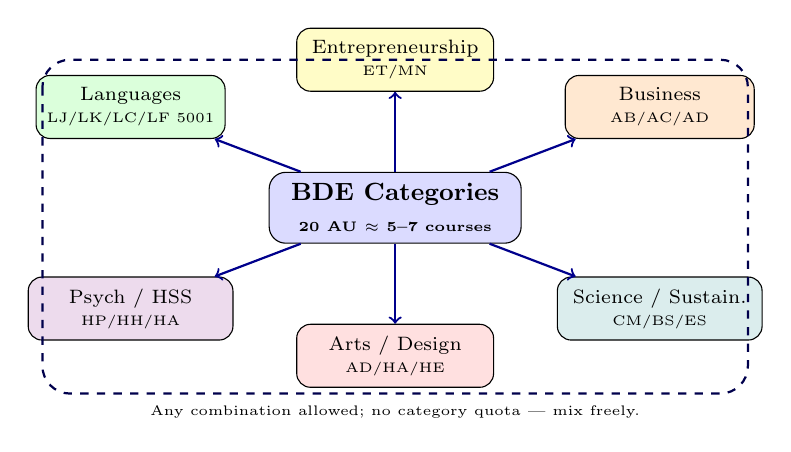
\begin{tikzpicture}[scale=0.80,every node/.style={font=\scriptsize}]
% Cloud-like grouping ellipses with colored fills
% Central anchor
\node[draw,fill=blue!14,rounded corners=6pt,minimum width=3.2cm,minimum height=0.9cm,align=center,font=\small\bfseries] (centre) at (0,0) {BDE Categories\\{\tiny 20 AU $\approx$ 5--7 courses}};
% Surrounding categories
\node[draw,fill=green!14,rounded corners=5pt,minimum width=2.4cm,minimum height=0.8cm,align=center] (lang) at (-4.2,1.6) {Languages\\{\tiny LJ/LK/LC/LF 5001}};
\node[draw,fill=orange!18,rounded corners=5pt,minimum width=2.4cm,minimum height=0.8cm,align=center] (biz) at (4.2,1.6) {Business\\{\tiny AB/AC/AD}};
\node[draw,fill=violet!14,rounded corners=5pt,minimum width=2.6cm,minimum height=0.8cm,align=center] (psych) at (-4.2,-1.6) {Psych / HSS\\{\tiny HP/HH/HA}};
\node[draw,fill=teal!14,rounded corners=5pt,minimum width=2.6cm,minimum height=0.8cm,align=center] (sci) at (4.2,-1.6) {Science / Sustain.\\{\tiny CM/BS/ES}};
\node[draw,fill=yellow!22,rounded corners=5pt,minimum width=2.5cm,minimum height=0.8cm,align=center] (ent) at (0,2.35) {Entrepreneurship\\{\tiny ET/MN}};
\node[draw,fill=red!12,rounded corners=5pt,minimum width=2.5cm,minimum height=0.8cm,align=center] (art) at (0,-2.35) {Arts / Design\\{\tiny AD/HA/HE}};
% Arrows from centre
\foreach \target in {lang,biz,psych,sci,ent,art} \draw[->,thick,blue!55!black] (centre) -- (\target);
% decorative cloud outline around outer nodes (approximate)
\draw[thick,dashed,blue!30!black,rounded corners=10pt] (-5.6,2.35) rectangle (5.6,-2.95);
\node[font=\tiny,fill=white,inner sep=2pt] at (0,-3.25) {Any combination allowed; no category quota --- mix freely.};
\end{tikzpicture}
\caption{BDE category cloud for NTU CS. No category is compulsory and no quota per category exists; breadth is the point. Second-major students will see this cloud shrink as BDE AU is repurposed.}
\label{fig:bde-cloud}
\end{figure}

No category is compulsory. A ``language + business + psychology'' mix is as valid as ``six entrepreneurship modules''. The only constraints are prerequisites (e.g., LJ5002 requires LJ5001), schedule clashes, and the double-count/exclusion rules above. Chapter~\ref{ch:planning} shows how to distribute these across four years.

\subsection{How to Verify for Your Cohort}
NTU curricula drift. The figures in this guide reflect the AY2024--25 CCDS CSC study plan (135~AU invariant) and NTUMods data at time of writing. For \emph{your} cohort:
\begin{enumerate}
    \item \textbf{Degree Audit} (StudentLink $\to$ Academic $\to$ Degree Audit) --- the single authoritative record. If this guide and Degree Audit disagree, Degree Audit wins.
    \item \textbf{CCDS curriculum page} (ntu.edu.sg/computing $\to$ Discover CCDS $\to$ Curriculum) --- bucket overview and study plan PDF.
    \item \textbf{NTUMods / Course Catalogue} (ntu.edu.sg $\to$ Education $\to$ Courses) --- per-course AU, prerequisites, exclusions, and whether a course is MPE-listed.
\end{enumerate}

% ============================================================
\section{Chapter Notes}
Curriculum buckets follow the CCDS BSc (Hons) in Computer Science programme structure (AY2024--25 study plan PDF and curriculum design page). AU definitions per NTU Academic Regulations. Historical GER terminology per NTU Curriculum Structure archives (pre-AY2021). Category examples drawn from NTU Course Catalogue listings at time of writing; offerings vary by semester.

% ============================================================
\section{Exercises}
\label{sec:ch01-exercises}
\begin{enumerate}[label=E1.\arabic*, leftmargin=*, itemsep=0.8em]
    \item \textbf{AU arithmetic.} You have completed 98~AU with 12~AU of BDE so far. How many BDE AU remain under the 20~AU bucket? If you add a second major requiring 28~AU that replaces BDE AU one-for-one, how many ``free'' BDE AU remain?
    \item \textbf{Double-count check.} You take SC4023 (AI for Software Engineering, 3~AU) listed as an MPE. Can you also count it toward BDE? What if SC4023 is \emph{not} on the MPE list for your cohort but you still take it --- does it count as BDE or neither?
    \item \textbf{Bucket invariant.} Explain why the two bucketings (curriculum page vs.\ PDF Foundational-Core summary) both sum to 135~AU despite showing BDE as 20 vs.\ 21.
    \item \textbf{Source triage.} A senior says ``BDE is 21~AU now''. Where do you verify, and which system is authoritative?
\end{enumerate}
% End of Chapter 1
